\subsection{GraphQL}
The main technology motivating this project is GraphQL, a query language developed by Facebook in 2012 \cite{byronKeynoteBriefHistory2019}.  This language, in comparison to querying languages such as SQL (Structured Query Language), is designed to be exposed as a public, web accessible, API.

\subsubsection{Language Structure}

The unique aspect of GraphQL that when data is requested from the API, the client requests the shape of the response.  What this means is that rather than the server defining the exact data that it will respond to the client with, the client has the freedom to adapt the data requested.

Another unique part of the language is that data accessible by the API is represented as a graph of connected data types.  You could imagine each type of requestable data being a node on a graph where the edges represent relationships between the data.  When combining the ability to dynamically request data from the server and being able to request related data, the power of GraphQL becomes evident.  Since the client requests exactly what it wants and can recieve all the related data in one request, the number of requests to the server is dramatically reduced and no extraneous data is sent to the client.

\begin{figure}[htbp]
    \centering
    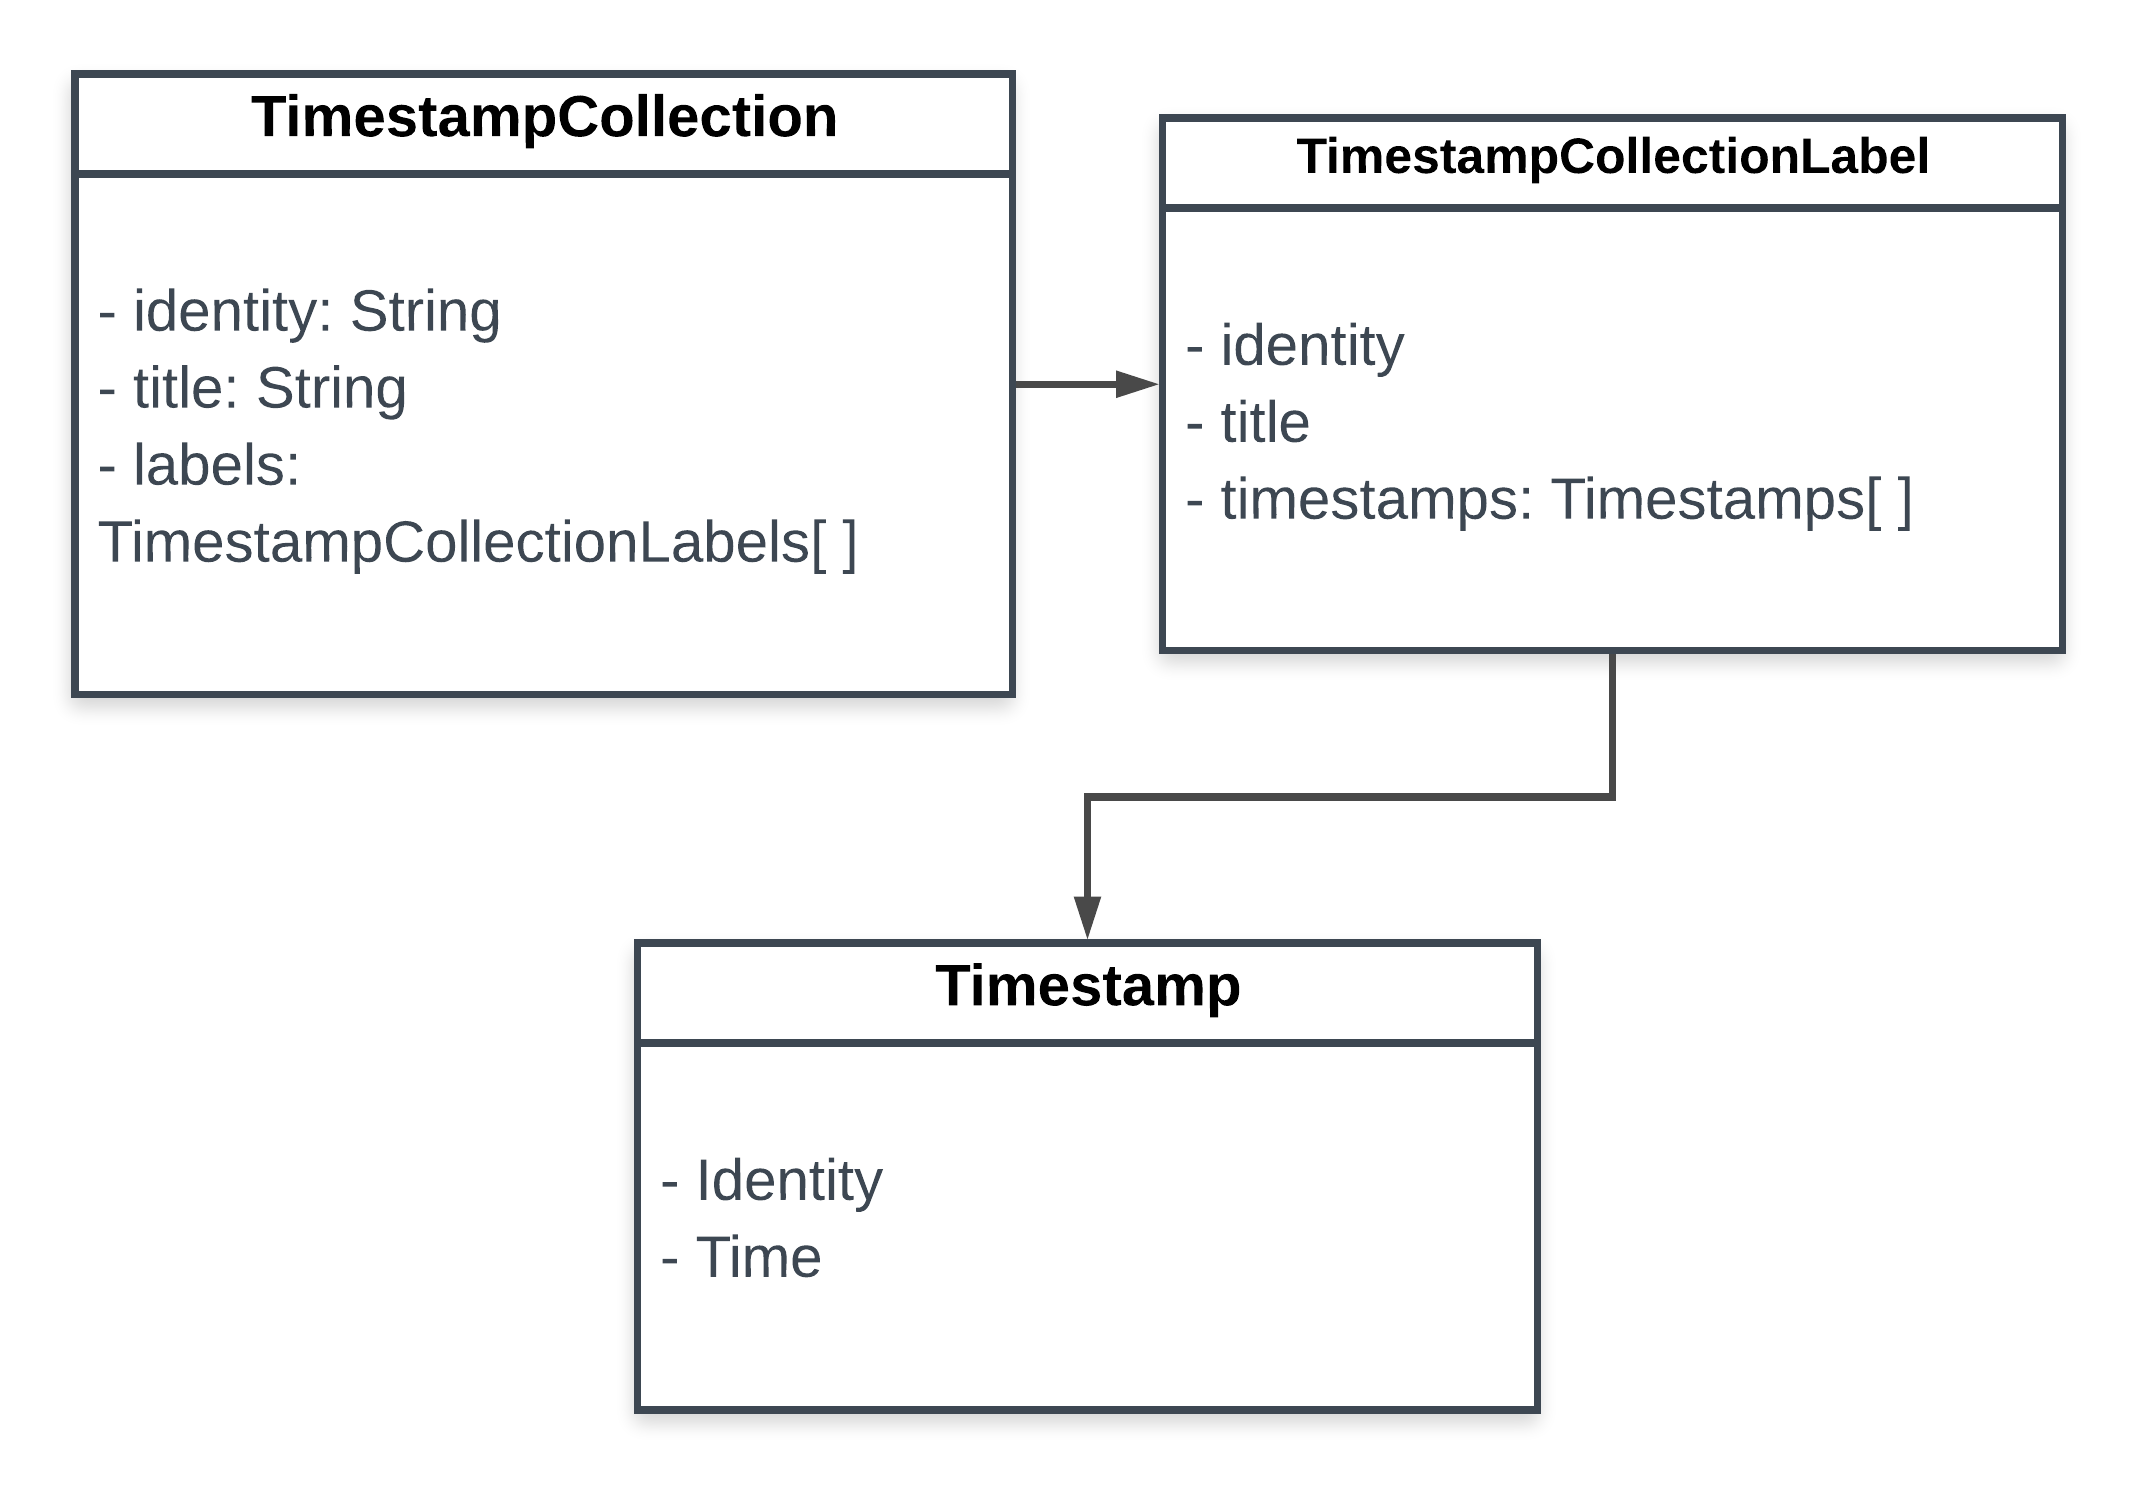
\includegraphics[scale=.15]{img/schema-graph.png}
    \caption{INSERT CAPTION HERE}
    \label{fig:schema-graph}
\end{figure}

Figure \ref{fig:schema-graph} is a visual representation of a GraphQL schema with three types, TimestampCollection, TimestampCollectionLabel, and Timestamp.  The relationships on this schema would allow the user to create a request as shown in Figure \ref{fig:basic-query}.  The result of this query would be all TimestampCollections with their associated labels and timestamps.  If not all the fields or connected data is need, however, any part of that query could be removed and the API would respond with less data.

\begin{figure}
    \begin{verbatim}
query {
    timestampCollections {
        identity
        title
        labels {
            title
            timestamps {
                time
            }
        }
    }
}
    \end{verbatim}
    \caption{A basic GraphQL query}
    \label{fig:basic-query}
\end{figure}

\subsubsection{GraphQL vs. SQL}

SQL is debatably one of the most popular querying languages thanks to the popularity of relational databases.  While the aim of this project is to connect GraphQL and SQL queries, it should be noted that the two languages exist for very different reasons.

SQL is a language very tied to the storage and retrival of data.  Queries act on specific tables that have strictly defined and structured data.  The SQL language does not make sense outside of the context of a relational database.  GraphQL on the other hand is completely agnostic to how the data is stored/retrieved.  The data source could be a relational database, a non-relational database, some other API, or could be programatically generated. To fetch and update all of this data, GraphQL servers implement resolvers that have the logic for that operation (whether that's accessing a database, running a function, or calling another service).  Because of this flexibility, it is possible to use GraphQL as the query language for the front end of the application and SQL as the query language used by a GraphQL server to fetch or update data in a database.